
\section{Wednesday for MAT3040}\index{Wednesday_lecture}
\subsection{Introduction to Tensor Product}
\paragraph{Reviewing}
Bilinear map: $f:V\times W\to U$, e.g.,
\[
\begin{array}{ll}
f:&\mathbb{R}^3\times\mathbb{R}^3\\
\text{with}&f(u,v)=u\times v
\end{array}
\]
Note that $f$ is usually not a linear transformation, e.g.,
\[
f(3(\bm v,\bm w)) = f(3\bm v,3\bm w) = (3\bm v)\times(3\bm w)=9\bm v\times\bm w\ne 3f(\bm v,\bm w).
\]

The vector space structure of $V\times W$ is not suited to study bilinear map, and the proper way is to study its induced linear transformation.

\begin{definition}[Universal Property of Tensor Product]
Let $V,W$ be vector spaces.
Consider the set
\[
\text{Obj}:=\{\phi:V\times W\to U\mid \text{$\phi$ is a bilinear map}\}
\]
We say $T$, or $(i:V\times W\to T)\in\text{Obj}$ satisfies the \emph{universal property} 
if for any $(\phi:V\times W\to T)\in\text{Obj}$, 
there exists an unique linear transformation $f_{\phi}:T\to U$ such that
the diagram below commutes:
\begin{figure}[H]
\centering
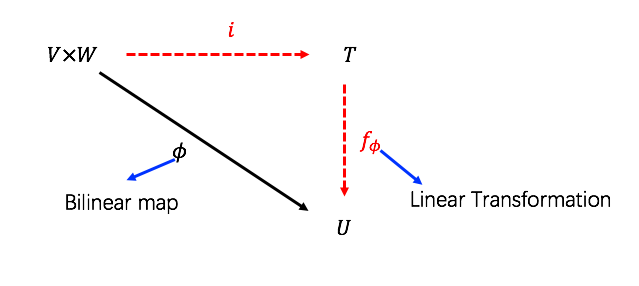
\includegraphics[width=0.5\textwidth]{week12/f_12_1}
\end{figure}
i.e., $\phi = f_{\phi}\circ i$.
\end{definition}
Therefore, rather than studying bilinear map $\phi$, it is better to study the linear transformation $f_\phi$ instead.

Question: does $T$ exist?

\begin{definition}[Spanning Set]
Let $V,W$ be vector spaces. Let $S = \{(\bm v,\bm w)\mid \bm v\in V,\bm w\in W\}$, then we define
\[
\mathfrak{X} = \Span(S).
\]
\end{definition}
\begin{remark}
\begin{enumerate}
\item
The spanning set $\mathfrak{X}$ is not addictive, e.g., $\mathfrak{x}_1=3(0,\bm w)\in\mathfrak{X}$ and $\mathfrak{x}_2=1(0,\bm w)+1(0,2\bm w)\in\mathfrak{X}$, but $\mathfrak{x}_1\ne\mathfrak{x}_2$.
\item
Note that we assume no relations on the elements $(\bm v,\bm w)\in\mathcal{S}$.
More precisely, the set $S=\{(\bm v,\bm w)\mid \bm v\in V,\bm w\in W\}$ is linearly independent in $\mathfrak{X}$.
For example, $(0,\bm w)\perp(0,2\bm w)$.
\item
The only legitimate relationship is
\[
2(\bm v_1,\bm w_1) + 3(\bm v_1,\bm w_1) = 5(\bm v,\bm w),
\]
which is not equal to $(5\bm v,5\bm w)$
\item
$\mathcal{S}$ is a basis of $\mathfrak{X}$, and therefore $\mathcal{X}$ is of uncountable dimension.
\end{enumerate}
\end{remark}

\begin{definition}[Special subspace of $\mathfrak{X}$]
Let ${y}\le\mathfrak{X}$ be a vector subspace spanned by vectors of the form
\[
\{1(\bm v_1,\bm v_2,\bm w) - 1(\bm v_1,\bm w) - 1(\bm v_2,\bm w)\},
\quad
\text{and}
\quad
\{1(\bm v,\bm w_1+\bm w_2) - 1(\bm v,\bm w_1) - 1(\bm v,\bm w_2)\}
\]
and
\[
\{1(k\bm v,\bm w) - k(\bm v,\bm w)\mid k\in\mathbb{F}\}
\]
and
\[
\{1(\bm v,k\bm w) - k(\bm v,\bm w)\mid k\in\mathbb{F}\}
\]
\end{definition}
\begin{definition}[Tensor Product]
We define the \emph{tensor product} $V\otimes W$ by 
\[
V\otimes W = \mathcal{X}/{y}.
\]
Therefore, $\bm v\otimes\bm w = (\bm v,\bm w)+{y}\in \mathcal{X}/{y}$
\end{definition}
\begin{remark}
\begin{enumerate}
\item
As a result, the tensor product is finitely addictive:
\begin{align*}
(\bm v_1+\bm v_2)\otimes\bm w&=(\bm v_1+\bm v_2,\bm w)+y\\
&=(\bm v_1+\bm v_2,\bm w)-[(\bm v_1+\bm v_2,\bm w) - (\bm v_1,\bm w) - (\bm v_2,\bm w)]+y\\
&=0(\bm v_1+\bm v_2,\bm w) + (\bm v_1,\bm w) + (\bm v_2,\bm w) + y\\
&=[(\bm v_1,\bm w)+y]+[(\bm v_2,\bm w)+y]\\
&=\bm v_1\otimes\bm w + \bm v_2\otimes\bm w
\end{align*}
Similarly, 
\begin{align*}
\bm v\otimes(\bm w_1+\bm w_2)&=(\bm v\otimes\bm w_1)+(\bm v\otimes\bm w_2)\\
(k\bm v)\otimes\bm w&=k(\bm v\otimes\bm w)\\
\bm v\otimes(k\bm w)&=k(\bm v\otimes\bm w)
\end{align*}
\item
The product space $V\times W$ is different from the tensor product space $V\otimes W$:
\begin{enumerate}
\item
$(\bm v,\bm0)\ne\bm0_{V\times W}$ in $V\times W$;
but $\bm v\otimes0\in 0_{V\otimes W}$:
\begin{align*}
V\otimes0&=V\otimes(0\bm w)\\
&=0(V\otimes w)\\
&=0_{V\otimes W}
\end{align*}
Moreover, $f$ is bilinear implies $f(\bm v,0)=\bm0$.
\item
$(\bm v_1,\bm w_1)+(\bm v_2,\bm w_2)=(\bm v_1+\bm v_2,\bm w_1+\bm w_2)$;
but $\bm v_1\otimes\bm w_1+\bm v_2\otimes\bm w_2$ cannot be simplified further, unless $\bm v_1=\bm v_2$:
\[
\bm v\otimes\bm w_1+\bm v\otimes\bm w_2 = \bm v\otimes(\bm w_1+\bm w_2)
\]
\end{enumerate}
\end{enumerate}
\end{remark}



\begin{theorem}\label{The:12:3}
The bilinear map
\[
\begin{array}{ll}
i:&V\times W\to V\otimes W\quad(i\in\text{Obj})\\
\text{with}&(\bm v,\bm w)\mapsto\bm v\otimes\bm w
\end{array}
\]
satisfies the universal property of tensor products.
\end{theorem}
\begin{example}
Consider a common bilinear map
\[
\begin{array}{ll}
\phi:&\mathbb{R}^3\times \mathbb{R}^3\to\mathbb{R}^3\\
\text{with}&(\bm v,\bm w)\mapsto\bm v\times\bm w
\end{array}
\]
By the universal property, there exists the linear transformation $f_{\phi}:\mathbb{R}^3\otimes\mathbb{R}^3\to\mathbb{R}^3$
such that the diagram below commutes:
\begin{figure}[H]
\centering
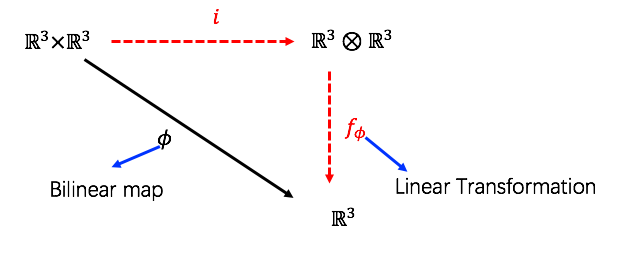
\includegraphics[width=0.6\textwidth]{week12/f_12_2}
\end{figure}
\end{example}













